\section{Path}

\subsection{Two Opposite Turns}

How the MPC takes advantage of subsequent opposite turns can be seen in Figure \ref{fig:paths_cur_150m}. When there is an opposite turn trailing the first turn, the optimized path cuts across the line connecting the two turns, while still keeping the camera on the observation path. This is also seen in Figure \ref{fig:paths_cur_heading} that shows the heading angle throughout the turn. The heading angle never reaches $45\degree$ or $70\degree$, because of cutting across the line.

\begin{figure}
	\makebox[\textwidth][c]{
	\subfloat[UAV position $45\degree$]{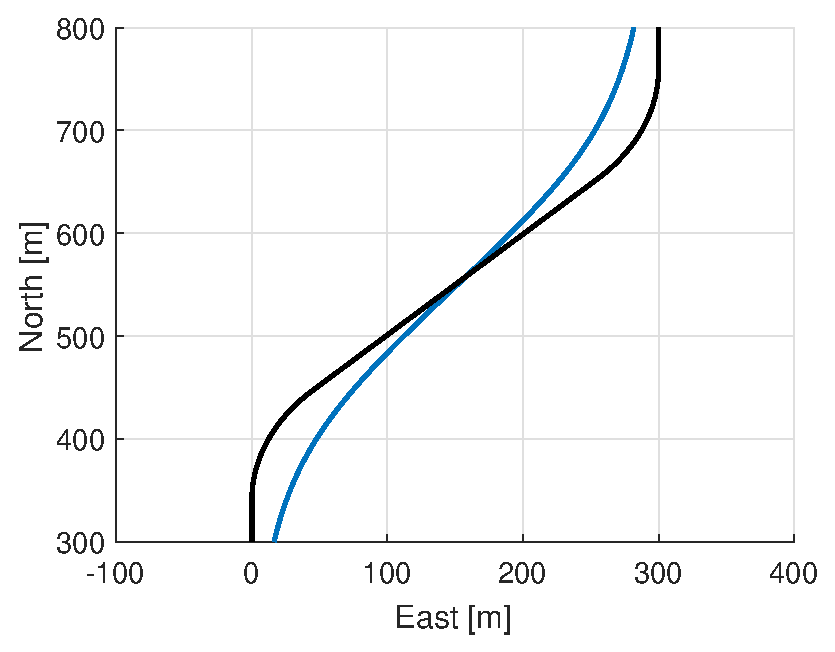
\includegraphics[width=0.5\textwidth, keepaspectratio=true]{../../results/opt/paths/fig_cur/uav_position_45deg_150m.eps}}
	\qquad
	\subfloat[UAV position $70\degree$]{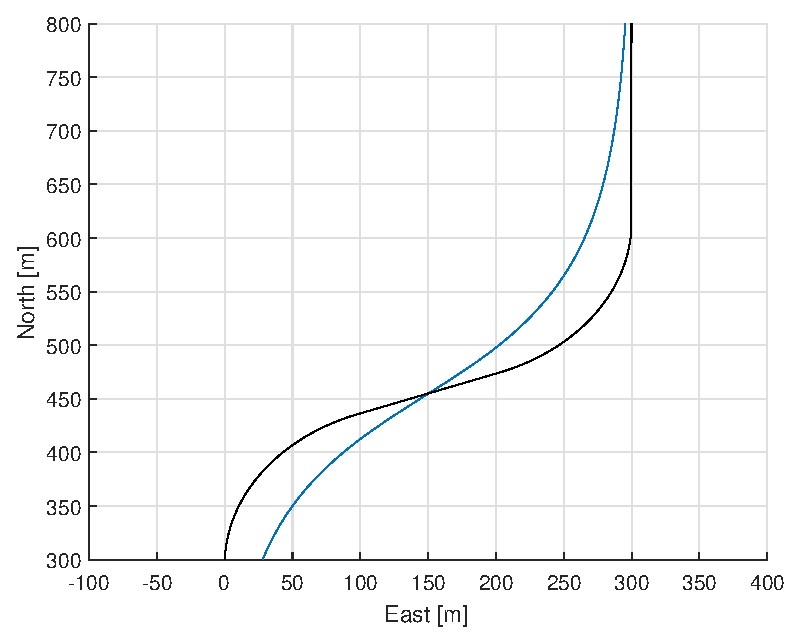
\includegraphics[width=0.5\textwidth, keepaspectratio=true]{../../results/opt/paths/fig_cur/uav_position_70deg_150m.eps}}}
	\makebox[\textwidth][c]{
	\subfloat[Camera position $45\degree$]{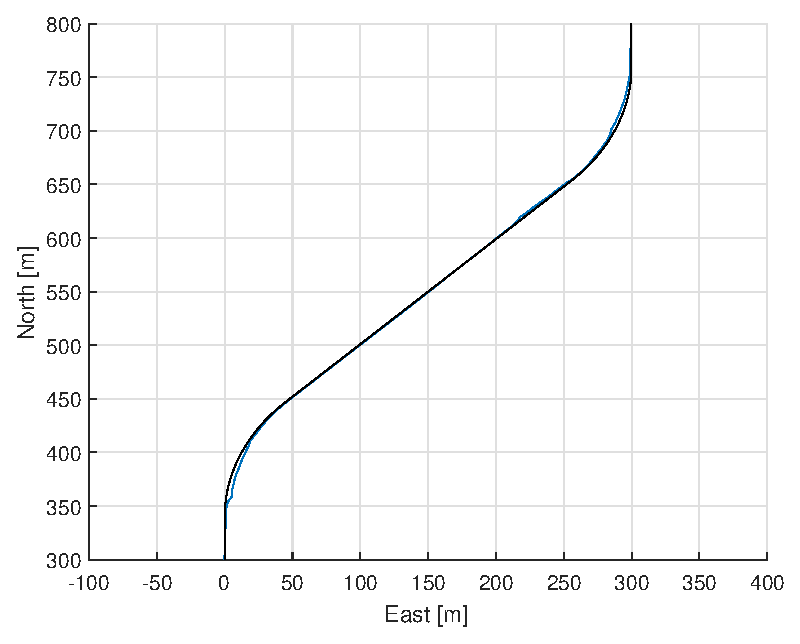
\includegraphics[width=0.5\textwidth, keepaspectratio=true]{../../results/opt/paths/fig_cur/camera_position_45deg_150m.eps}}
	\qquad
	\subfloat[Camera position $70\degree$]{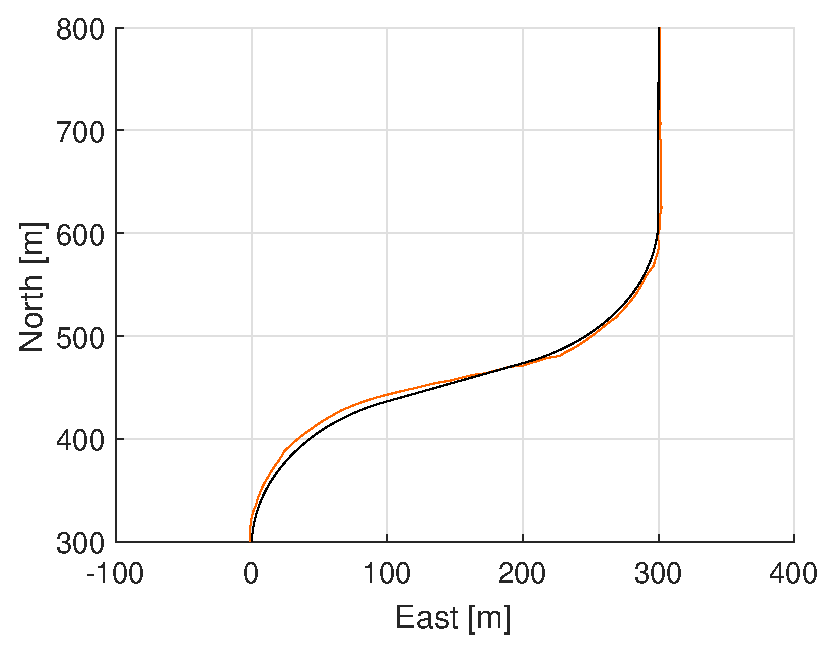
\includegraphics[width=0.5\textwidth, keepaspectratio=true]{../../results/opt/paths/fig_cur/camera_position_70deg_150m.eps}}}
	\makebox[\textwidth][c]{
	\subfloat[Heading angle]{\includegraphics[width=0.5\textwidth, keepaspectratio=true]{../../results/opt/paths/fig_cur/heading.eps}
	\label{fig:paths_cur_heading}}}
	\caption{UAV position, camera position and heading angle during two subsequent turns of $45\degree$ and $70\degree$.}
	\label{fig:paths_cur_150m}
\end{figure}